\let\negmedspace\undefined
\let\negthickspace\undefined
\documentclass[journal,12pt,onecolumn]{IEEEtran}
\usepackage{cite}
\usepackage{amsmath,amssymb,amsfonts,amsthm}
\usepackage{algorithmic}
\usepackage{graphicx}
\graphicspath{{./figs/}}
\usepackage{textcomp}
\usepackage{xcolor}
\usepackage{txfonts}
\usepackage{listings}
\usepackage{enumitem}
\usepackage{mathtools}
\usepackage{gensymb}
\usepackage{comment}
\usepackage{caption}
\usepackage[breaklinks=true]{hyperref}
\usepackage{tkz-euclide} 
\usepackage{listings}
\usepackage{gvv}                                        
%\def\inputGnumericTable{}                                 
\usepackage[latin1]{inputenc}     
\usepackage{xparse}
\usepackage{color}                                            
\usepackage{array}                                            
\usepackage{longtable}                                       
\usepackage{calc}                                             
\usepackage{multirow}
\usepackage{multicol}
\usepackage{hhline}                                           
\usepackage{ifthen}                                           
\usepackage{lscape}
\usepackage{tabularx}
\usepackage{array}
\usepackage{float}
\newtheorem{theorem}{Theorem}[section]
\newtheorem{problem}{Problem}
\newtheorem{proposition}{Proposition}[section]
\newtheorem{lemma}{Lemma}[section]
\newtheorem{corollary}[theorem]{Corollary}
\newtheorem{example}{Example}[section]
\newtheorem{definition}[problem]{Definition}
\newcommand{\BEQA}{\begin{eqnarray}}
\newcommand{\EEQA}{\end{eqnarray}}
\newcommand{\define}{\stackrel{\triangle}{=}}
\theoremstyle{remark}
\newtheorem{rem}{Remark}

\begin{document}
\title{
ASSIGNMENT 4: GATE 2020 \\
    PH : PHYSICS }
\author{AI25BTECH11035 - Sujal Rajani }
\maketitle
\renewcommand{\thefigure}{\theenumi}
\renewcommand{\thetable}{\theenumi}
\textbf{Q1-Q5 carry one mark each} 
\begin{enumerate}
    

\item He is known for his unscrupulous ways. He always sheds \underline{\hspace{1cm}} tears to deceive people.
   
    \begin{enumerate}
        \item fox's
        \item crocodile's
        \item crocodile
        \item fox
    \end{enumerate}
    

    \item Jofra Archer, the England fast bowler, is \underline{\hspace{1cm}} than accurate.
   
    \begin{enumerate}
        \item more fast
        \item faster
        \item less fast
        \item more faster
    \end{enumerate}
   
    \item Select the word that fits the analogy: \\
    Build : Building :: Grow : \underline{\hspace{1cm}}
   
    \begin{enumerate}
        \item Grown
        \item Grew
        \item Growth
        \item Growed
    \end{enumerate}
    

    \item I do not think you know the case well enough to have opinions. Having said that, I agree with your other point.\\
    What does the phrase "having said that" mean in the given text?
    \begin{enumerate}
        \item as opposed to what I have said
        \item despite what I have said
        \item in addition to what I have said
        \item contrary to what I have said
    \end{enumerate}
    

    \item Define $[x]$ as the greatest integer less than or equal to $x$, for each $x \in (-\infty, \infty)$. If $y = [x]$, then area under $y$ for $x \in [1,4]$ is \underline{\hspace{1cm}}.
    
    \begin{enumerate}
        \item 1
        \item 3
        \item 4
        \item 6
    \end{enumerate}
    

    \textbf{Q6-Q10 carry two mark each}
    \item \textbf{Crowd funding deals with mobilisation of funds for a project from a large number of people, who would be willing to invest smaller amounts through web-based platforms in the project.}\\
    Based on the above paragraph, which of the following is correct about crowd funding?
    
    \begin{enumerate}
        \item Funds raised through unwilling contributions on web-based platforms.
        \item Funds raised through large contributions on web-based platforms.
        \item Funds raised through coerced contributions on web-based platforms.
        \item Funds raised through voluntary contributors on non web-based platforms.
    \end{enumerate}
    \item P, Q, R and S are to be uniquely coded using $\alpha$ and $\beta$. If P is coded as $\alpha\alpha$ and Q as $\alpha\beta$, then R and S, respectively, can be coded as \underline{\hspace{2cm}}.
    
    \begin{enumerate}
        \item $\beta\alpha$ and $\alpha\beta$
        \item $\beta\beta$ and $\alpha\alpha$
        \item $\alpha\beta$ and $\beta\beta$
        \item $\beta\alpha$ and $\beta\beta$
    \end{enumerate}
    
    \item The sum of the first $n$ terms in the sequence $8,88, 888, 8888,\dots$ is .
    
    \begin{enumerate}
        \item $ \frac{81}{80} (10^n - 1) + \frac{9}{8} n$
        \item $ \frac{81}{80} (10^n - 1) - \frac{9}{8} n$
        \item $ \frac{80}{81} (10^n - 1) + \frac{8}{9} n$
        \item $\frac{80}{81} (10^n - 1) - \frac{8}{9} n$
    \end{enumerate}
    
    
    \item Select the graph that schematically represents BOTH $y = x^m$ and $y = x^{1/m}$ properly in the interval $0 \leq x \leq 1$, for integer values of $m$, where $m > 1$.
    \begin{figure}[H]
    \centering
    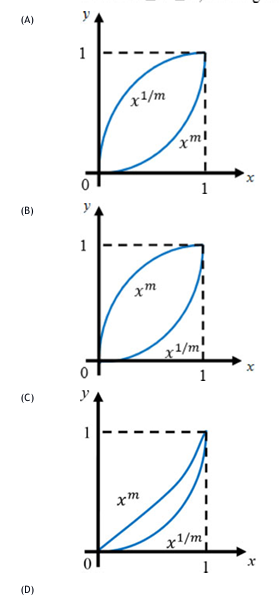
\includegraphics[width=0.25\columnwidth]{fig/Q9(1).png}
     \caption*{}
    \label{fig:Q43}
\end{figure}
\begin{figure}[H]
    \centering
    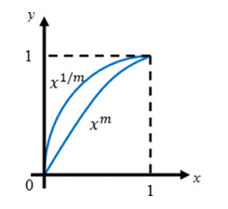
\includegraphics[width=0.25\columnwidth]{fig/Q9(2).png}
     \caption*{}
    \label{fig:Q43}
\end{figure}
    \item The bar graph shows the data of the students who appeared and passed in an examination for four schools P, Q, R and S. The average of success rates (in percentage) of these four schools is \underline{\hspace{2cm}}.
  \begin{figure}[H]
    \centering
    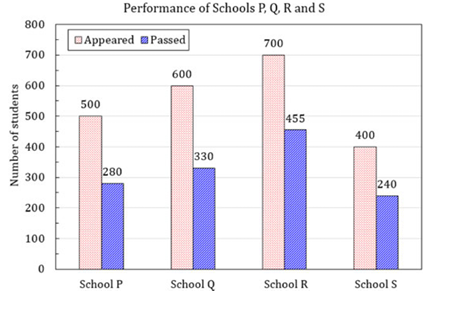
\includegraphics[width=0.5\columnwidth]{fig/Q10.png}
     \caption*{}
    \label{fig:Q10}
\end{figure}
    
    \begin{enumerate}
        \item 58.5 \%
        \item 58.8 \%
        \item 59.0 \%
        \item 59.3 \%
    \end{enumerate}
    
\end{enumerate}

\section*{PH: Physics}
\subsection*{Q1 - Q25 carry one mark each.}

\begin{enumerate}
    \item Which one of the following is a solution of
    $ \dfrac{d^2 u(x)}{dx^2} = k^2 u(x)$, for k real?
    
    
    \begin{enumerate} 
        \item $e^{-kx}$
        \item $\sin kx$
        \item $\cos kx$
        \item $\sin x$
    \end{enumerate}
   

    \item A real, invertible $3 \times 3$ matrix $M$ has eigenvalues $\lambda_i$, ($i=1,2,3$) and the corresponding eigenvectors are $|e_i\rangle$, ($i=1,2,3$) respectively. Which one of the following is correct?
   
    \begin{enumerate}
        \item $M |e_i\rangle = \frac{1}{\lambda_i} |e_i\rangle$, for $i = 1,2,3$
        \item $M^{-1} |e_i\rangle = \frac{1}{\lambda_i} |e_i\rangle$, for $i = 1,2,3$
        \item $M^{-1}|e_i\rangle = \lambda_i |e_i\rangle$, for $i = 1,2,3$
        \item The eigenvalues of $M$ and $M^{-1}$ are not related.
    \end{enumerate}
    
    \item A quantum particle is subjected to the potential
    \begin{align}
          V(x) = \begin{cases}
            \infty, & x \leq -\frac{a}{2} \\
            0, & -\frac{a}{2} < x < \frac{a}{2} \\
            \infty, & x \geq \frac{a}{2}
        \end{cases}
     \end{align}
    The ground state wave function of the particle is proportional to
    
    \begin{enumerate}
        \item $\sin\brak{\dfrac{\pi x}{2a}}$
        \item $\sin\brak{k\dfrac{\pi x}{a}}$
        \item $\cos\brak{\dfrac{\pi x}{2a}}$
        \item $\cos\brak{\dfrac{\pi x}{a}}$
    \end{enumerate}
   

    \item Let $\hat{a}$ and $\hat{a}^\dagger$, respectively, denote the lowering and raising operators of a one-dimensional simple harmonic oscillator. Let $|n\rangle$ be the energy eigenstate of the simple harmonic oscillator. Given that $|n\rangle$ is also an eigenstate of $\hat{a}^\dagger \hat{a}^\dagger \hat{a} \hat{a}$, the corresponding eigenvalue is
    
    \begin{enumerate}
        \item $n(n-1)$
        \item $n(n+1)$
        \item $(n+1)^2$
        \item $n^2$
    \end{enumerate}
    

    \item Which one of the following is a universal logic gate?
   
    \begin{enumerate}
        \item AND
        \item NOT
        \item OR
        \item NAND
    \end{enumerate}
    

    \item Which one of the following is the correct binary equivalent of the hexadecimal F6C?
    
    \begin{enumerate}
        \item 0110 1111 1100
        \item 1111 0110 1100
        \item 1100 0110 1111
        \item 0110 1100 0111
    \end{enumerate}
    

    \item The total angular momentum $j$ of the ground state of the ${}^{17}_{8}$O nucleus is
    
    \begin{enumerate}
        \item $\dfrac{1}{2}$
        \item $1$
        \item $\dfrac{3}{2}$
        \item $\dfrac{5}{2}$
    \end{enumerate}
    
    \item A particle $X$ is produced in the process $\pi^+ + p \rightarrow K^+ + X$ via the strong interaction. If the quark content of the $K^+$ is $u\bar{s}$, the quark content of $X$ is
   
    \begin{enumerate}
        \item $c\bar{s}$
        \item $uud$
        \item $uu\bar{s}$
        \item $u\bar{d}$
    \end{enumerate}
   

    \item A medium ($\epsilon_r > 1$, $\mu_r = 1$, $\sigma > 0$) is semi-transparent to an electromagnetic wave when
    
    \begin{enumerate}
        \item Conduction current $\gg$ Displacement current
        \item Conduction current $\ll$ Displacement current
        \item Conduction current = Displacement current
        \item Both Conduction current and Displacement current are zero
    \end{enumerate}
   

    \item A particle is moving in a central force field given by $\vec{F} = -\dfrac{k}{r^3}\hat{r}$, where $\hat{r}$ is the unit vector pointing away from the center of the field. The potential energy of the particle is given by
    
    \begin{enumerate}
        \item $\dfrac{k}{r^2}$
        \item $\dfrac{k}{2r^2}$
        \item $-\dfrac{k}{r^2}$
        \item $\dfrac{k}{2r^2}$
    \end{enumerate}
    

    \item Choose the correct statement related to the Fermi energy ($E_F$) and the chemical potential ($\mu$) of a metal.
    
    \begin{enumerate}
        \item $\mu = E_F$ only at $0$ K
        \item $\mu = E_F$ at finite temperature
        \item $\mu < E_F$ at $0$ K
        \item $\mu > E_F$ at finite temperature
    \end{enumerate}
    

    \item Consider a diatomic molecule formed by identical atoms. If $E_v$ and $E_e$ represent the energy of the vibrational nuclear motion and electronic motion respectively, then in terms of the electronic mass $m$ and nuclear mass $M$, $\dfrac{E_v}{E_e}$ is proportional to
   
    \begin{enumerate}
        \item $\brak{\dfrac{m}{M}}^{1/2}$
        \item $\dfrac{m}{M}$
        \item $\brak{\dfrac{m}{M}}^{3/2}$
        \item $\brak{\dfrac{m}{M}}^{2}$
    \end{enumerate}
    
    \item Which one of the following relations determines the manner in which the electric field lines are refracted across the interface between two dielectric media having dielectric constants $\varepsilon_1$ and $\varepsilon_2$ (see figure)?
 \begin{figure}[H]
    \centering
    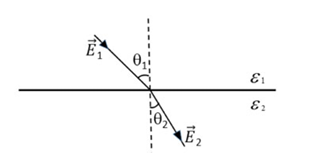
\includegraphics[width=0.4\columnwidth]{fig/Q13.png}
     \caption*{}
    \label{fig:Q13}
\end{figure}
    \begin{enumerate}
        \item $\varepsilon_1 \sin\theta_1 = \varepsilon_2 \sin\theta_2$
        \item $\varepsilon_1 \cos\theta_1 = \varepsilon_2 \cos\theta_2$
        \item $\varepsilon_1 \tan\theta_1 = \varepsilon_2 \tan\theta_2$
        \item $\varepsilon_1 \cot\theta_1 = \varepsilon_2 \cot\theta_2$
    \end{enumerate}
    

    \item If $\vec{E}$ and $\vec{B}$ are the electric and magnetic fields respectively, then $\vec{E} \cdot \vec{B}$ is
   
    \begin{enumerate}
        \item odd under parity and even under time reversal
        \item even under parity and odd under time reversal
        \item odd under parity and odd under time reversal
        \item even under parity and even under time reversal
    \end{enumerate}
    

    \item A small disc is suspended by a fiber such that it is free to rotate about the fiber axis (see figure). For small angular deflections, the Hamiltonian for the disc is given by
    \begin{align}
        H = \frac{p_\theta^2}{2I} + \frac{1}{2}\alpha\theta^2,
    \end{align}
    where $I$ is the moment of inertia and $\alpha$ is the restoring torque per unit deflection. The disc is subjected to angular deflections ($\theta$) due to thermal collisions from the surrounding gas at temperature $T$ and $p_\theta$ is the momentum conjugate to $\theta$. The average and the root-mean-square angular deflection, $\theta_{avg}$ and $\theta_{{rms}}$, respectively are
\begin{figure}[H]
    \centering
    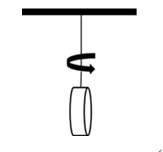
\includegraphics[width=0.25\columnwidth]{fig/Q15.png}
     \caption*{}
    \label{fig:Q15}
\end{figure}
  
    \begin{multicols}{2}
    \begin{enumerate}
        \item $\theta_{{avg}} = 0$ and $\theta_{{rms}} = \brak{\dfrac{k_B T}{\alpha}}^{3/2}$
        \item $\theta_{{avg}} = 0$ and $\theta_{{rms}} = \brak{\dfrac{k_B T}{\alpha}}^{1/2}$
        \item $\theta_{{avg}} \neq 0$ and $\theta_{{rms}} = \brak{\dfrac{k_B T}{\alpha}})^{1/2}$
        \item $\theta_{{avg}} \neq 0$ and $\theta_{{rms}} = \brak{\dfrac{k_B T}{\alpha}}^{3/2}$
    \end{enumerate}
    \end{multicols}
     \item As shown in the figure, an ideal gas is confined to chamber A of an insulated container, with vacuum in chamber B. When the plug in the wall separating the chambers A and B is removed, the gas fills both the chambers. Which one of the following statements is true?
     \begin{figure}[H]
    \centering
    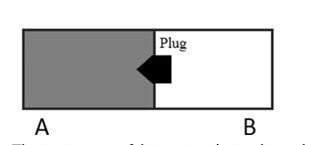
\includegraphics[width=0.25\columnwidth]{fig/Q16.png}
     \caption*{}
    \label{fig:Q16}
\end{figure}
   
    \begin{enumerate}
        \item The temperature of the gas remains unchanged
        \item Internal energy of the gas decreases
        \item Temperature of the gas decreases as it expands to fill the space in chamber B
        \item Internal energy of the gas increases as its atoms have more space to move around
    \end{enumerate}
    
    
    \item Particle A with angular momentum $j = \frac{3}{2}$ decays into two particles B and C with angular momenta $j_1$ and $j_2$, respectively. If $|2, \frac{3}{2}\rangle_A = \alpha |1,1\rangle_B \otimes |1, \frac{1}{2}\rangle_C$, the value of $\alpha$ is \underline{\hspace{2cm}}.

    \item Far from the Earth, the Earth's magnetic field can be approximated as due to a bar magnet of magnetic pole strength $4 \times 10^{14}$ Am. Assume this magnetic field is generated by a current carrying loop encircling the magnetic equator. The current required to do so is about $4 \times 10^n$ A, where $n$ is an integer. The value of $n$ is \underline{\hspace{2cm}}.\\
    (Earth's circumference: $4 \times 10^7$ m)

    \item The number of distinct ways the primitive unit cell can be constructed for the two dimensional lattice as shown in the figure is \underline{\hspace{2cm}}.
    \begin{figure}[H]
    \centering
    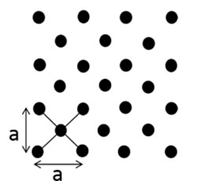
\includegraphics[width=0.25\columnwidth]{fig/Q19.png}
     \caption*{}
    \label{fig:Q19}
\end{figure}
   

    \item A hydrogenic atom is subjected to a strong magnetic field. In the absence of spin-orbit coupling, the number of doubly degenerate states created out of the d-level is \underline{\hspace{2cm}}.

    \item A particle $Y$ undergoes strong decay $Y \rightarrow \pi^+ + \pi^-$. The isospin of $Y$ is \underline{\hspace{2cm}}.
\item For a complex variable $z$ and the contour $c:|z|=1$ taken in the counter clockwise direction,
    $
        \frac{1}{2\pi i} \oint_c \brak{z - 2 + \frac{3}{z^2}} dz = \underline{\hspace{2cm}}
    $
    
    \item Let $p$ be the momentum conjugate to the generalized coordinate $q$. If the transformation
    \begin{align}
        Q = \sqrt{2} q^m \cos p \\
        P = \sqrt{2} q^m \sin p
    \end{align}
    is canonical, then $m =$ \underline{\hspace{2cm}}
    
    \item A conducting sphere of radius $1$ m is placed in air. The maximum number of electrons that can be put on the sphere to avoid electrical breakdown is about $7 \times 10^n$, where $n$ is an integer. The value of $n$ is \underline{\hspace{2cm}}
    
    
    Breakdown electric field strength in air is $|\vec{E}|=3 \times 10^6~\text{V/m}$ \\
   perm of free space  $\epsilon_0 = 8.85 \times 10^{-12}{F/m}$\\
    Electron charge $ e = 1.60 \times 10^{-19}C$

    
    
    \item If a particle is moving along a sinusoidal curve, the number of degrees of freedom of the particle is \underline{\hspace{2cm}}
    
    \textbf{Q26-Q55 carry two marks each }
    
    \item The product of eigenvalues of
    $
        \myvec{
            0 & 0 & 1 \\
            0 & 1 & 0 \\
            1 & 0 & 0}
    $
    is
    
    \begin{enumerate}
        \item $-1$
        \item $1$
        \item $0$
        \item $2$
    \end{enumerate}
    

    \item Let $|e_1\rangle = \myvec{1\\0\\0}$, $|e_2\rangle = \myvec{1\\1\\0}$ and $|e_3\rangle = \myvec{1\\1\\1}$. Let $S = \{|e_1\rangle, |e_2\rangle, |e_3\rangle\}$. Let $\mathbb{R}^3$ denote the three-dimensional real vector space. Which one of the following is correct?
    
    \begin{enumerate}
        \item $S$ is an orthonormal set
        \item $S$ is a linearly dependent set
        \item $S$ is a basis for $\mathbb{R}^3$
        \item $\sum_{i=1}^3|e_i\rangle\langle e_i|=
        \myvec{
            1 & 0 & 0\\
            0 & 1 & 0\\
            0 & 0 & 1}
        $
    \end{enumerate}
    
    \item $\hat{S}_x$ denotes the spin operator defined as $\hat{S}_x = \dfrac{\hbar}{2}\myvec{0 & 1 \\ 1 & 0}$. Which one of the following is correct?
    
    \begin{enumerate}
        \item The eigenstates of spin operator $\hat{S}_x$ are $|\uparrow\rangle_x = \myvec{1\\0}$ and $|\downarrow\rangle_x = \myvec{0\\1}$
        \item The eigenstates of spin operator $\hat{S}_x$ are $|\uparrow\rangle_x = \frac{1}{\sqrt{2}}\myvec{1\\-1}$ and $|\downarrow\rangle_x = \frac{1}{\sqrt{2}},\myvec{1\\1}$
        \item In the spin state $\dfrac{1}{2}\myvec{1\\\sqrt{3}}$, upon the measurement of $\hat{S}_x$, the probability for obtaining $|\uparrow\rangle_x$ is $\dfrac{1}{4}$
        \item In the spin state $\dfrac{1}{2}\myvec{1\\\sqrt{3}}$, upon the measurement of $\hat{S}_x$, the probability for obtaining $|\uparrow\rangle_x$ is $\dfrac{2+\sqrt{3}}{4}$
    \end{enumerate}
    
    
    \item The input voltage ($V_{\text{in}}$) to the circuit shown in the figure is $2\cos(100t)$ V. The output voltage ($V_{\text{out}}$) is $2\cos\left(100t - \frac{\pi}{2}\right)$ V. If $R = 1$ k$\Omega$, the value of $C$ (in $\mu$F) is
     \begin{figure}[H]
    \centering
    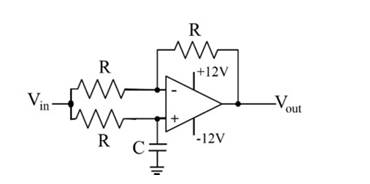
\includegraphics[width=0.5\columnwidth]{fig/Q29.png}
     \caption*{}
    \label{fig:Q19}
\end{figure}
   
    \begin{enumerate}
        \item 0.1
        \item 1
        \item 10
        \item 100
    \end{enumerate}
    
     \item Consider a 4-bit counter constructed out of four flip-flops. It is formed by connecting the J and K inputs to logic high and feeding the Q output to the clock input of the following flip-flop (see the figure). The input signal to the counter is a series of square pulses and the change of state is triggered by the falling edge. At time $t = t_0$ the outputs are in logic low state ($Q_0 = Q_1 = Q_2 = Q_3 = 0$). Then at $t = t_1$, the logic state of the outputs is
    \begin{figure}[H]
    \centering
    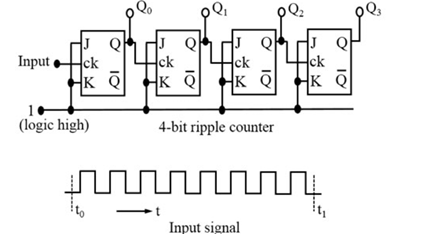
\includegraphics[width=0.5\columnwidth]{fig/Q30.png}
     \caption*{}
    \label{fig:Q30}
\end{figure}
   
    \begin{enumerate}
        \item $Q_0 = 1$, $Q_1 = 0$, $Q_2 = 0$ and $Q_3 = 0$
        \item $Q_0 = 0$, $Q_1 = 0$, $Q_2 = 0$ and $Q_3 = 1$
        \item $Q_0 = 1$, $Q_1 = 0$, $Q_2 = 1$ and $Q_3 = 0$
        \item $Q_0 = 0$, $Q_1 = 1$, $Q_2 = 1$ and $Q_3 = 1$
    \end{enumerate}
    

    \item Consider the Lagrangian
    $
        L = a \brak{\frac{dx}{dt}}^2 + b\brak{\frac{dy}{dt}}^2 + cxy
    $
    where $a$, $b$ and $c$ are constants. If $p_x$ and $p_y$ are the momenta conjugate to the coordinates $x$ and $y$ respectively, then the Hamiltonian is
    
    \begin{enumerate}
        \item $\dfrac{p_x^2}{4a} + \dfrac{p_y^2}{4b} - cxy$
        \item $\dfrac{p_x^2}{2a} + \dfrac{p_y^2}{2b} - cxy$
        \item $\dfrac{p_x^2}{2a} + \dfrac{p_y^2}{2b} + cxy$
        \item $\dfrac{p_x^2}{a} + \dfrac{p_y^2}{b} + cxy$
    \end{enumerate}
    

    \item Which one of the following matrices does NOT represent a proper rotation in a plane?
    
    \begin{enumerate}
        \item $
        \myvec{
        -\sin\theta & \cos\theta \\
        -\cos\theta & -\sin\theta
        }
        $
        \item $
        \myvec{
        \cos\theta & \sin\theta \\
        -\sin\theta & \cos\theta
        }
        $
        \item $
        \myvec{
        \sin\theta & \cos\theta \\
        \cos\theta & \sin\theta
        }
        $
        \item $
        \myvec{
        -\cos\theta & \sin\theta \\
        -\sin\theta & \cos\theta
        }$
    \end{enumerate}
    
     \item A uniform magnetic field $\vec{B} = B_0 \hat{y}$ exists in an inertial frame $K$. A perfect conducting sphere moves with a constant velocity $\vec{v} = v_0 \hat{x}$ with respect to this inertial frame. The rest frame of the sphere is $K'$ (see figure). The electric and magnetic fields in $K$ and $K'$ are related as
    
    \begin{align}
    \vec{E}'_{||} &= \vec{E}_{||} \qquad \vec{E}'_{\perp} = \gamma\brak{\vec{E}_{\perp} + \vec{v} \times \vec{B}}  \\
    \vec{B}'_{||} &= \vec{B}_{||} \qquad
    \vec{B}'_{\perp} = \gamma \brak{ \vec{B}_{\perp} - \frac{\vec{v}}{c^2} \times \vec{E}}
    \end{align}
    $\qquad
    \gamma = \frac{1}{\sqrt{1 - (v/c)^2}}$
    
    The induced surface charge density on the sphere (to the lowest order in $v/c$) in the frame $K'$ is
    \begin{figure}[H]
    \centering
    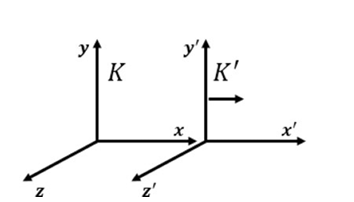
\includegraphics[width=0.25\columnwidth]{fig/Q33.png}
     \caption*{}
    \label{fig:Q33}
\end{figure}
   
    
    \begin{enumerate}
        \item maximum along $z'$
        \item maximum along $y'$
        \item maximum along $x'$
        \item uniform over the sphere
    \end{enumerate}
    

    \item A charge $q$ moving with uniform speed enters a cylindrical region in free space at $t=0$ and exits the region at $t = \tau$ (see figure). Which one of the following options best describes the time dependence of the total electric flux $\varphi(t)$, through the entire surface of the cylinder?
   \begin{figure}[H]
    \centering
    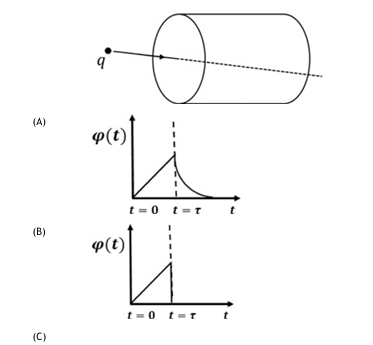
\includegraphics[width=0.5\columnwidth]{fig/Q34(1).png}
     \caption*{}
    \label{fig:Q34(1)}
\end{figure}
   \begin{figure}[H]
    \centering
    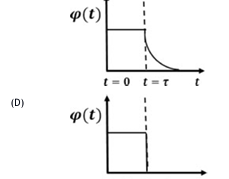
\includegraphics[width=0.4\columnwidth]{fig/Q34(2).png}
     \caption*{}
    \label{fig:Q34(2)}
\end{figure}
   
   
     \item Consider a one-dimensional non-magnetic crystal with one atom per unit cell. Assume that the valence electrons (i) do not interact with each other and (ii) interact weakly with the ions. If $n$ is the number of valence electrons per unit cell, then at $0$ K,
    
    \begin{enumerate}
        \item the crystal is metallic for any value of $n$
        \item the crystal is non-metallic for any value of $n$
        \item the crystal is metallic for even values of $n$
        \item the crystal is metallic for odd values of $n$
    \end{enumerate}
   

    \item According to the Fermi gas model of the nucleus, the nucleons move in a spherical volume of radius $R (= R_0 A^{1/3})$, where $A$ is the mass number and $R_0$ is an empirical constant with the dimensions of length. The Fermi energy of the nucleus $E_F$ is proportional to
    
    \begin{enumerate}
        \item $R_0^2$
        \item $\dfrac{1}{R_0}$
        \item $\dfrac{1}{R_0^2}$
        \item $\dfrac{1}{R_0^3}$
    \end{enumerate}
    
    \item Consider a two dimensional crystal with $3$ atoms in the basis. The number of allowed optical branches ($n$) and acoustic branches ($m$) due to the lattice vibrations are
   
    \begin{enumerate}
        \item $(n, m) = (2, 4)$
        \item $(n, m) = (3, 3)$
        \item $(n, m) = (4, 2)$
        \item $(n, m) = (1, 5)$
    \end{enumerate}
    

    \item The internal energy $U$ of a system is given by $U(S, V) = \lambda V^{-2/3} S^2$, where $\lambda$ is a constant of appropriate dimensions; $V$ and $S$ denote the volume and entropy, respectively. Which one of the following gives the correct equation of state of the system?
    
    \begin{enumerate}
        \item $P V^{1/3} T^2 = \text{constant}$
        \item $\dfrac{P V}{T} = \text{constant}$
        \item $P V T^{1/3} = \text{constant}$
        \item $\dfrac{P V^2}{T} = \text{constant}$
    \end{enumerate}
    
    \item The potential energy of a particle of mass $m$ is given by
    $
        U(x) = a \sin (k^2 x - \pi/2), \quad a > 0,\quad k^2 > 0.
    $
    The angular frequency of small oscillations of the particle about $x=0$ is
    
    \begin{enumerate}
        \item $k^2 \sqrt{\dfrac{2a}{m}}$
        \item $k^2 \sqrt{\dfrac{a}{m}}$
        \item $k^2 \sqrt{\dfrac{a}{2m}}$
        \item $2k^2 \sqrt{\dfrac{a}{m}}$
    \end{enumerate}
    

    \item The radial wave function of a particle in a central potential is given by
    $
        R(r) = A \dfrac{r}{a} \exp\brak{-\dfrac{r}{2a}}
    $,where $A$ is the normalization constant and $a$ is positive constant of suitable dimensions. If $\gamma a$ is the most probable distance of the particle from the force center, the value of $\gamma$ is \underline{\hspace{2cm}}
    
    \item A free particle of mass $M$ is located in a three-dimensional cubic potential well with impenetrable walls. The degeneracy of the fifth excited state of the particle is \underline{\hspace{2cm}}
    
    \item Consider the circuit given in the figure. Let the forward voltage drop across each diode be $0.7$ V. The current I (in mA) through the resistor is \underline{\hspace{2cm}}
    \begin{figure}[H]
    \centering
    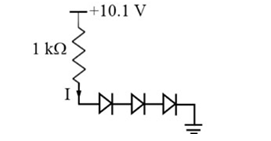
\includegraphics[width=0.25\columnwidth]{fig/Q42.png}
     \caption*{}
    \label{fig:Q42}
\end{figure}
    \item Let $u^\mu$ denote the 4-velocity of a relativistic particle whose square $u^\mu u_\mu = 1$. If $\epsilon_{\mu\nu\rho\sigma}$ is the Levi-Civita tensor then the value of $\epsilon_{\mu\nu\rho\sigma}u^\mu u^\nu u^\rho u^\sigma$ is \underline{\hspace{2cm}}
    \item Consider a simple cubic monoatomic Bravais lattice which has a basis with vectors $\vec{r}_1 = 0$, $\vec{r}_2 = \dfrac{a}{4}(\hat{x} + \hat{y} + \hat{z})$, $a$ is the lattice parameter. The Bragg reflection is observed due to the change in the wave vector between the incident and the scattered beam as given by $\vec{K} = n_1\vec{G}_1 + n_2\vec{G}_2 + n_3\vec{G}_3$, where $\vec{G}_1$, $\vec{G}_2$ and $\vec{G}_3$ are primitive reciprocal lattice vectors. For $n_1 = 3$, $n_2 = 3$ and $n_3 = 2$, the geometrical structure factor is \underline{\hspace{2cm}}
    
    \item A plane electromagnetic wave of wavelength $\lambda$ is incident on a circular loop of conducting wire. The loop radius is $a$ ($a << \lambda$). The angle (in degrees), made by the Poynting vector with the normal to the plane of the loop to generate a maximum induced electrical signal, is \underline{\hspace{2cm}}
    
    \item An electron in a hydrogen atom is in the state $n=3, l=2, m=-2$. Let $\hat{L}_y$ denote the y-component of the orbital angular momentum operator. If $(\Delta \hat{L}_y)^2 = a\hbar^2$, the value of $a$ is \underline{\hspace{2cm}}
    
    \item A sinusoidal voltage of the form $V(t)=V_0\cos(\omega t)$ is applied across a parallel plate capacitor placed in vacuum. Ignoring the edge effects, the induced $\mathrm{emf}$ within the region between the capacitor plates can be expressed as a power series in $\omega$. The lowest non-vanishing exponent in $\omega$ is \underline{\hspace{2cm}}
    
    \item If $x = \sum_{k=1}^{\infty} a_k \sin k x$, for $-\pi \leq x \leq \pi$, the value of $a_2$ is \underline{\hspace{2cm}}
    
    \item Let $f_n(x) = \begin{cases}
        0, & x < -\frac{1}{2n}\\
        n, & -\frac{1}{2n} < x < \frac{1}{2n}\\
        0, & \frac{1}{2n} < x
    \end{cases}$

    The value of $\lim_{n \rightarrow \infty} \int_{-\infty}^{\infty} f_n(x)\sin x dx$ is \underline{\hspace{2cm}}
    
    \item Consider the Hamiltonian $\hat{H} = \hat{H}_0 + \hat{H}'$ where
    \begin{align}
        \hat{H}_0 =
       \myvec{
            E & 0 & 0 \\
            0 & E & 0 \\
            0 & 0 & E
        }
        \end{align}
        and $\hat{H}'$ is the independent perturbation given by
        
        \begin{align}
        \hat{H}' =
        \myvec{
            0 & k & 0 \\
            k & 0 & k \\
            0 & k & 0}
        \end{align}
    , where $k > 0$. If the maximum energy eigenvalue of $\hat{H}$ is $3$ eV corresponding to $E = 2$ eV, the value of $k$ (rounded off to three decimal places) in eV is \underline{\hspace{2cm}}
    \item A hydrogen atom is in an orbital angular momentum state $|l,m = l \rangle$. If $\vec{L}$ lies on a cone which makes a half angle $30^\circ$ with respect to the $z$-axis, the value of $l$ is \underline{\hspace{2cm}}
    
    \item In the center of mass frame, two protons each having energy $7000$ GeV, collide to produce protons and anti-protons. The maximum number of anti-protons produced is \underline{\hspace{2cm}}.\\
    (Assume the proton mass to be $1$ GeV$/c^2$)

    \item Consider a gas of hydrogen atoms in the atmosphere of the Sun where the temperature is $5800$ K. If a sample from this atmosphere contains $6.023 \times 10^{23}$ of hydrogen atoms in the ground state, the number of hydrogen atoms in the first excited state is approximately $8 \times 10^n$, where $n$ is an integer. The value of $n$ is \underline{\hspace{2cm}}.\\
    (Boltzmann constant: $8.617 \times 10^{-5}$ eV/K)
    
    \item For a gas of non-interacting particles, the probability that a particle has a speed $v$ in the interval $v$ to $v+dv$ is given by
    \begin{align}
        f(v) dv = 4\pi v^2 dv \left(\frac{m}{2\pi k_B T}\right)^{3/2} e^{-mv^2/2k_B T}
    \end{align}
    If $E$ is the energy of a particle, then the maximum in the corresponding energy distribution in units of $E/k_B T$ occurs at \underline{\hspace{2cm}} (rounded off to one decimal place).
    
    \item The Planck's energy density distribution is given by
    \begin{align}
        u(\omega) = \dfrac{h \omega^3}{\pi^2 c^3} \dfrac{1}{e^{h\omega/k_B T} - 1}
    \end{align}
    At long wavelengths, the energy density of photons in thermal equilibrium with a cavity at temperature $T$ varies as $T^\alpha$, where $\alpha$ is \underline{\hspace{2cm}}
    \end{enumerate}
    \end{document}
    